

\tikzset{every picture/.style={line width=0.75pt}} %set default line width to 0.75pt        

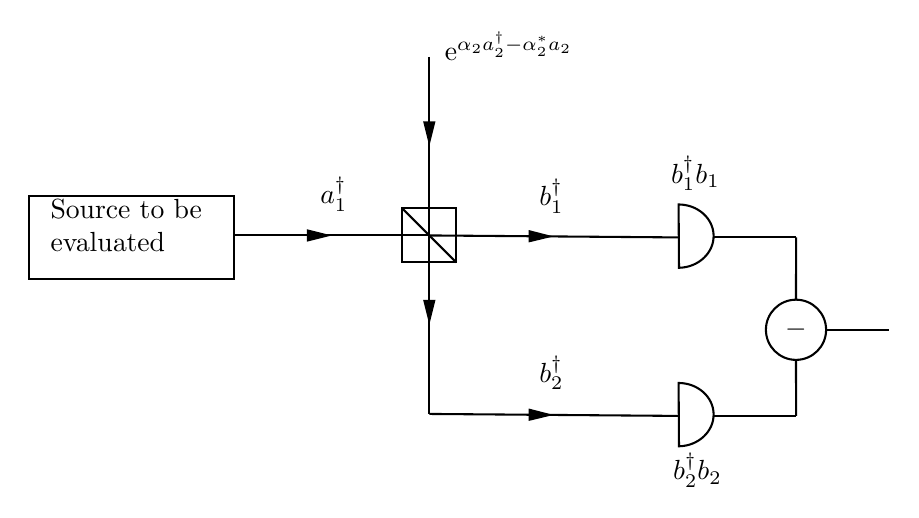
\begin{tikzpicture}[x=0.75pt,y=0.75pt,yscale=-1,xscale=1]
%uncomment if require: \path (0,300); %set diagram left start at 0, and has height of 300

%Shape: Square [id:dp48465100337411604] 
\draw   (286,119) -- (260,119) -- (260,145) -- (286,145) -- cycle ;
%Straight Lines [id:da009730264904362462] 
\draw    (286,145) -- (260,119) ;

%Straight Lines [id:da841426330546053] 
\draw    (179,132) -- (273,132) ;
\draw [shift={(226,132)}, rotate = 180] [fill={rgb, 255:red, 0; green, 0; blue, 0 }  ][line width=0.08]  [draw opacity=0] (12,-3) -- (0,0) -- (12,3) -- cycle    ;
%Straight Lines [id:da3980567150516523] 
\draw    (273,46) -- (273,132) ;
\draw [shift={(273,89)}, rotate = 270] [fill={rgb, 255:red, 0; green, 0; blue, 0 }  ][line width=0.08]  [draw opacity=0] (12,-3) -- (0,0) -- (12,3) -- cycle    ;
%Straight Lines [id:da7111057972380808] 
\draw    (273,132) -- (273,218) ;
\draw [shift={(273,175)}, rotate = 270] [fill={rgb, 255:red, 0; green, 0; blue, 0 }  ][line width=0.08]  [draw opacity=0] (12,-3) -- (0,0) -- (12,3) -- cycle    ;
%Straight Lines [id:da12521956138792478] 
\draw    (273,132) -- (392.71,132.95) ;
\draw [shift={(332.85,132.48)}, rotate = 180.46] [fill={rgb, 255:red, 0; green, 0; blue, 0 }  ][line width=0.08]  [draw opacity=0] (12,-3) -- (0,0) -- (12,3) -- cycle    ;
%Shape: Chord [id:dp14603723174788152] 
\draw   (393.11,117.08) .. controls (402.31,117.1) and (409.82,123.7) .. (409.98,132) .. controls (410.14,140.42) and (402.68,147.4) .. (393.3,147.58) -- cycle ;
%Straight Lines [id:da09107409379680376] 
\draw    (273,218) -- (392.71,218.95) ;
\draw [shift={(332.85,218.48)}, rotate = 180.46] [fill={rgb, 255:red, 0; green, 0; blue, 0 }  ][line width=0.08]  [draw opacity=0] (12,-3) -- (0,0) -- (12,3) -- cycle    ;
%Shape: Chord [id:dp158377588748835] 
\draw   (393.11,203.08) .. controls (402.31,203.1) and (409.82,209.7) .. (409.98,218) .. controls (410.14,226.42) and (402.68,233.4) .. (393.3,233.58) -- cycle ;
%Straight Lines [id:da39545292367915774] 
\draw    (409.71,132.95) -- (449.71,132.95) ;
%Straight Lines [id:da29050927155087436] 
\draw    (409.71,218.95) -- (449.71,218.95) ;
%Straight Lines [id:da4259702929343543] 
\draw    (449.71,132.95) -- (449.68,162.95) ;
%Straight Lines [id:da376644991684453] 
\draw    (449.68,191.95) -- (449.71,218.95) ;
%Shape: Circle [id:dp47795417904392656] 
\draw   (435.18,177.45) .. controls (435.18,169.45) and (441.67,162.95) .. (449.68,162.95) .. controls (457.69,162.95) and (464.18,169.45) .. (464.18,177.45) .. controls (464.18,185.46) and (457.69,191.95) .. (449.68,191.95) .. controls (441.67,191.95) and (435.18,185.46) .. (435.18,177.45) -- cycle ;
%Straight Lines [id:da9614966812921062] 
\draw    (464.18,177.45) -- (494.71,177.45) ;
%Shape: Rectangle [id:dp9974767092600316] 
\draw   (80,113) -- (179,113) -- (179,153) -- (80,153) -- cycle ;

% Text Node
\draw (279,32.4) node [anchor=north west][inner sep=0.75pt]    {$\mathrm{e}^{\alpha_{2} a^\dagger_2 - \alpha^*_2 a_2}$};
% Text Node
\draw (324.5,103.4) node [anchor=north west][inner sep=0.75pt]    {$b_{1}^{\dagger }$};
% Text Node
\draw (324.5,188.4) node [anchor=north west][inner sep=0.75pt]    {$b_{2}^{\dagger }$};
% Text Node
\draw (449.68,177.45) node    {$-$};
% Text Node
\draw (388,92.4) node [anchor=north west][inner sep=0.75pt]    {$\expval{b_1^\dagger b_1}$};
% Text Node
\draw (389,235.4) node [anchor=north west][inner sep=0.75pt]    {$\expval{b_2^\dagger b_2}$};
% Text Node
\draw (89,113) node [anchor=north west][inner sep=0.75pt]   [align=left] {Source to be \\evaluated};
% Text Node
\draw (219,102.4) node [anchor=north west][inner sep=0.75pt]    {$a_{1}^{\dagger }$};


\end{tikzpicture}
